\documentclass{article}
\usepackage[utf8]{inputenc}
\usepackage[T1]{fontenc}
\usepackage{listings}
\usepackage{booktabs}
\usepackage{xcolor}
\usepackage{graphicx}
\usepackage[margin=1in]{geometry}
\usepackage{upquote}
\usepackage{textcomp}
\DeclareUnicodeCharacter{2502}{\textbar{}}
\DeclareUnicodeCharacter{2500}{-}
\DeclareUnicodeCharacter{253C}{+}
\DeclareUnicodeCharacter{252C}{+}
\DeclareUnicodeCharacter{2534}{+}
\DeclareUnicodeCharacter{251C}{+}
\DeclareUnicodeCharacter{2524}{+}
\DeclareUnicodeCharacter{250C}{+}
\DeclareUnicodeCharacter{2510}{+}
\DeclareUnicodeCharacter{2514}{+}
\DeclareUnicodeCharacter{2518}{+}
\lstset{upquote=true,extendedchars=true,literate={│}{{\textbar{}}}1 {─}{{-}}1 {┼}{{+}}1 {┬}{{+}}1 {┴}{{+}}1 {├}{{+}}1 {┤}{{+}}1 {┌}{{+}}1 {┐}{{+}}1 {└}{{+}}1 {┘}{{+}}1 {ä}{{\"a}}1 {ö}{{\"o}}1 {ü}{{\"u}}1 {Ä}{{\"A}}1 {Ö}{{\"O}}1 {Ü}{{\"U}}1 {ß}{{\ss}}1 {é}{{\'e}}1 {è}{{\`e}}1 {ê}{{\^e}}1 {ë}{{\"e}}1 {É}{{\'E}}1 {á}{{\'a}}1 {à}{{\`a}}1 {â}{{\^a}}1 {í}{{\'i}}1 {ì}{{\`i}}1 {î}{{\^i}}1 {ï}{{\"i}}1 {ó}{{\'o}}1 {ò}{{\`o}}1 {ô}{{\^o}}1 {ú}{{\'u}}1 {ù}{{\`u}}1 {û}{{\^u}}1 {ñ}{{\~n}}1 {ç}{{\c c}}1 {å}{{\r a}}1 {Å}{{\r A}}1 {æ}{{\ae}}1 {Æ}{{\AE}}1 {ø}{{\o}}1 {Ø}{{\O}}1 {±}{{\ensuremath{\pm}}}1 {°}{{\textdegree}}1 {µ}{{\textmu}}1 {×}{{\ensuremath{\times}}}1 {–}{{-}}1 {—}{{--}}1 {≤}{{\ensuremath{\le}}}1 {≥}{{\ensuremath{\ge}}}1}

\definecolor{statacommand}{RGB}{0,85,170}
\definecolor{stataerror}{RGB}{192,57,43}
\definecolor{stataoutput}{RGB}{73,80,87}
\definecolor{statabg}{RGB}{248,249,250}

\lstset{
  basicstyle=\ttfamily\small,
  breaklines=true,
  breakatwhitespace=false,
  columns=fullflexible,
  keepspaces=true,
  showstringspaces=false,
  frame=none,
  xleftmargin=0.5em,
}

\lstdefinestyle{statacommand}{
  basicstyle=\ttfamily\small\color{statacommand},
  backgroundcolor=\color{statabg},
  frame=l,
  framerule=2pt,
  rulecolor=\color{statacommand},
}

\lstdefinestyle{stataoutput}{
  basicstyle=\ttfamily\footnotesize\color{stataoutput},
}

\lstdefinestyle{stataerror}{
  basicstyle=\ttfamily\footnotesize\color{stataerror},
}

\title{LaTeX Export Example}
\date{28 April 2026}
\author{}

\begin{document}
\maketitle

\section{Data Overview}

\begin{lstlisting}[style=statacommand]
. summarize price mpg weight length, separator(0)
\end{lstlisting}

\begin{lstlisting}[style=stataoutput]
    Variable │        Obs        Mean    Std. dev.       Min        Max
─────────────┼─────────────────────────────────────────────────────────
       price │         74    6165.257    2949.496       3291      15906
         mpg │         74     21.2973    5.785503         12         41
      weight │         74    3019.459    777.1936       1760       4840
      length │         74    187.9324    22.26634        142        233

\end{lstlisting}

\begin{lstlisting}[style=statacommand]
. tabstat price mpg weight, by(foreign) statistics(n mean sd median min max) columns(statistics)
\end{lstlisting}

\begin{lstlisting}[style=stataoutput]
Summary for variables: price mpg weight
Group variable: foreign (Car origin)

 foreign │         N      Mean        SD       p50       Min       Max
─────────┼────────────────────────────────────────────────────────────
Domestic │        52  6072.423  3097.104    4782.5      3291     15906
         │        52  19.82692  4.743297        19        12        34
         │        52  3317.115  695.3637      3360      1800      4840
─────────┼────────────────────────────────────────────────────────────
 Foreign │        22  6384.682  2621.915      5759      3748     12990
         │        22  24.77273  6.611187      24.5        14        41
         │        22  2315.909  433.0035      2180      1760      3420
─────────┼────────────────────────────────────────────────────────────
   Total │        74  6165.257  2949.496    5006.5      3291     15906
         │        74   21.2973  5.785503        20        12        41
         │        74  3019.459  777.1936      3190      1760      4840
─────────┴────────────────────────────────────────────────────────────

\end{lstlisting}

\section{Regression Analysis}

\begin{lstlisting}[style=statacommand]
. regress price mpg weight length i.foreign
\end{lstlisting}

\begin{lstlisting}[style=stataoutput]
      Source │       SS           df       MS      Number of obs   =        74
─────────────┼──────────────────────────────────   F(4, 69)        =     21.01
       Model │   348708940         4    87177235   Prob > F        =    0.0000
    Residual │   286356456        69  4150093.57   R-squared       =    0.5491
─────────────┼──────────────────────────────────   Adj R-squared   =    0.5230
       Total │   635065396        73  8699525.97   Root MSE        =    2037.2

\end{lstlisting}

\begin{verbatim}
─────────────┬────────────────────────────────────────────────────────────────
       price │ Coefficient  Std. err.      t    P>|t|     [95% conf. interval]
─────────────┼────────────────────────────────────────────────────────────────
         mpg │  -13.40719   72.10761    -0.19   0.853    -157.2579    130.4436
      weight │   5.716181   1.016095     5.63   0.000     3.689127    7.743235
      length │  -92.48018    33.5912    -2.75   0.008    -159.4928   -25.46758
             │
     foreign │
    Foreign  │   3550.194   655.4564     5.42   0.000     2242.594    4857.793
       _cons │    5515.58   5241.941     1.05   0.296    -4941.807    15972.97
─────────────┴────────────────────────────────────────────────────────────────
\end{verbatim}

\begin{lstlisting}[style=statacommand]
. estimates store base
\end{lstlisting}

\subsection{Margins}

\begin{lstlisting}[style=statacommand]
. margins foreign, atmeans
\end{lstlisting}

\begin{lstlisting}[style=stataoutput]

Adjusted predictions                                        Number of obs = 74
Model VCE: OLS

Expression: Linear prediction, predict()
At: mpg       =  21.2973 (mean)
    weight    = 3019.459 (mean)
    length    = 187.9324 (mean)
    0.foreign = .7027027 (mean)
    1.foreign = .2972973 (mean)

\end{lstlisting}

\begin{verbatim}
─────────────┬────────────────────────────────────────────────────────────────
             │            Delta-method
             │     Margin   std. err.      t    P>|t|     [95% conf. interval]
─────────────┼────────────────────────────────────────────────────────────────
     foreign │
   Domestic  │   5109.794   306.6837    16.66   0.000     4497.977    5721.611
    Foreign  │   8659.987   517.9058    16.72   0.000     7626.794    9693.181
─────────────┴────────────────────────────────────────────────────────────────
\end{verbatim}

\section{Tabulations}

\begin{lstlisting}[style=statacommand]
. tabulate foreign rep78, row
\end{lstlisting}

\begin{lstlisting}[style=stataoutput]
┌────────────────┐
│ Key            │
├────────────────┤
│   frequency    │
│ row percentage │
└────────────────┘

           │                   Repair record 1978
Car origin │         1          2          3          4          5 │     Total
───────────┼───────────────────────────────────────────────────────┼──────────
  Domestic │         2          8         27          9          2 │        48
           │      4.17      16.67      56.25      18.75       4.17 │    100.00
───────────┼───────────────────────────────────────────────────────┼──────────
   Foreign │         0          0          3          9          9 │        21
           │      0.00       0.00      14.29      42.86      42.86 │    100.00
───────────┼───────────────────────────────────────────────────────┼──────────
     Total │         2          8         30         18         11 │        69
           │      2.90      11.59      43.48      26.09      15.94 │    100.00

\end{lstlisting}

\section{Diagnostics}

\begin{lstlisting}[style=statacommand]
. quietly regress price mpg weight
\end{lstlisting}

\begin{lstlisting}[style=statacommand]
. predict double resid, residuals
\end{lstlisting}

\begin{lstlisting}[style=statacommand]
. histogram resid, normal ///
>     title("Residual Distribution") ///
>     xtitle("Residuals") ytitle("Density")
\end{lstlisting}

\begin{lstlisting}[style=stataoutput]
(bin=8, start=-3332.4617, width=1354.9264)

\end{lstlisting}

\begin{lstlisting}[style=statacommand]
. graph export "logdoc/demo/residuals.png", replace width(900)
\end{lstlisting}

\begin{figure}[htbp]
\centering
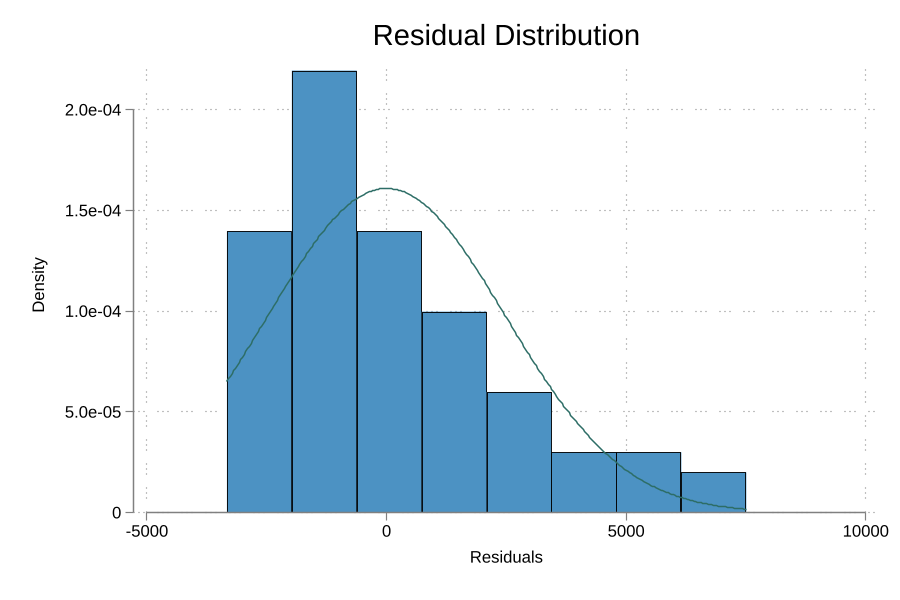
\includegraphics[width=0.8\textwidth]{residuals.png}
\end{figure}

\begin{lstlisting}[style=stataoutput]
file logdoc/demo/residuals.png written in PNG format

\end{lstlisting}

\begin{lstlisting}[style=statacommand]
. capture graph close _all
\end{lstlisting}

\begin{lstlisting}[style=statacommand]
. drop resid
\end{lstlisting}


\end{document}
